Consider the $m$-degree polynomial $P(m, X, N)$ having fixed non-negative integers $m$ and $N$
\begin{align*}
    P(m,X,N) = \sum_{r=0}^{m} \sum_{k=1}^{N} \coeffA{m}{r} k^r (X-k)^r
\end{align*}
For example
\begin{align*}
    P(2,X,0) &= 0 \\
    P(2,X,1) &= 30X^2 - 60X + 31 \\
    P(2,X,2) &= 150X^2 - 540X + 512 \\
    P(2,X,3) &= 420X^2 - 2160X + 2943 \\
    P(2,X,4) &= 900X^2 - 6000X + 10624
\end{align*}
where $\coeffA{m}{r}$ is a real coefficient defined recursively, see~\cite{alekseyev2018mathoverflow,
    on_the_link_between_binomial_theorem_and_discrete_convolution, unusual_identity_for_odd_powers,
    history_and_overview_of_polynomial_p}.
For example,
\begin{table}[H]
    \begin{center}
        \setlength\extrarowheight{-6pt}
        \begin{tabular}{c|cccccccc}
            $m/r$ & 0 & 1       & 2      & 3      & 4   & 5    & 6     & 7 \\ [3px]
            \hline
            0     & 1 &         &        &        &     &      &       &       \\
            1     & 1 & 6       &        &        &     &      &       &       \\
            2     & 1 & 0       & 30     &        &     &      &       &       \\
            3     & 1 & -14     & 0      & 140    &     &      &       &       \\
            4     & 1 & -120    & 0      & 0      & 630 &      &       &       \\
            5     & 1 & -1386   & 660    & 0      & 0   & 2772 &       &       \\
            6     & 1 & -21840  & 18018  & 0      & 0   & 0    & 12012 &       \\
            7     & 1 & -450054 & 491400 & -60060 & 0   & 0    & 0     & 51480
        \end{tabular}
    \end{center}
    \caption{Coefficients $\coeffA{m}{r}$. See OEIS sequences
    ~\cite{oeis_numerators_of_the_coefficient_a_m_r,oeis_denominators_of_the_coefficient_a_m_r}.}
    \label{tab:table_of_coefficients_a}
\end{table}


The polynomial $P(m, X, N)$ is derived from a rearrangement of Faulhaber's formula
in the context of Knuth's work entitled \textit{Johann Faulhaber and sums of powers}, see~\cite{knuth1993johann}.
In particular, the polynomial $P(m, X, N)$ yields an identity for odd powers
\begin{align*}
    P(m, X, X) = X^{2m+1}
\end{align*}
In its extended form
\begin{align*}
    X^{2m+1} = \sum_{r=0}^{m} \sum_{k=1}^{X} \coeffA{m}{r} k^r (X-k)^r
\end{align*}
The exact relation between Faulhaber's formula and $P(m,X,N)$ is shown by~\cite{kolosov2025unexpected}.

However, apart from the polynomial identity for odd powers, a few approximation properties of $P(m,X,N)$
were discovered in addition.
Therefore, in this manuscript we explore the approximation properties of the polynomial $P(m,X,N)$.
During our discussion, we utilize the following well-known criteria to measure and estimate
the error of approximation: Absolute error, Relative error and Percentage error.
Assume that the function $f_2(x)$ approximates the function $f_1 (x)$, then errors are given by
\begin{align*}
    \mathrm{Absolute \; Error}   &= \lvert f_1(x) - f_2(x) \rvert \\
    \mathrm{Relative \; Error}   &= \frac{\lvert f_1(x) - f_2(x) \rvert}{\lvert f_1(x) \rvert} \\
    \mathrm{Percentage \; Error} &= \frac{\lvert f_1(x) - f_2(x) \rvert}{\lvert f_1(x) \rvert} \times 100\%
\end{align*}

Diving straight into the point, we switch our focus to the partial case of polynomial
$P(2,X,4) = 900X^2 - 6000X + 10624$
to show the first example of how it approximates the odd power function $X^5$.
In general, we approximate the polynomial $X^{2m+1}$ using a lower-degree polynomial of degree $m$,
as shown in the following image
\begin{figure}[H]
    \centering
    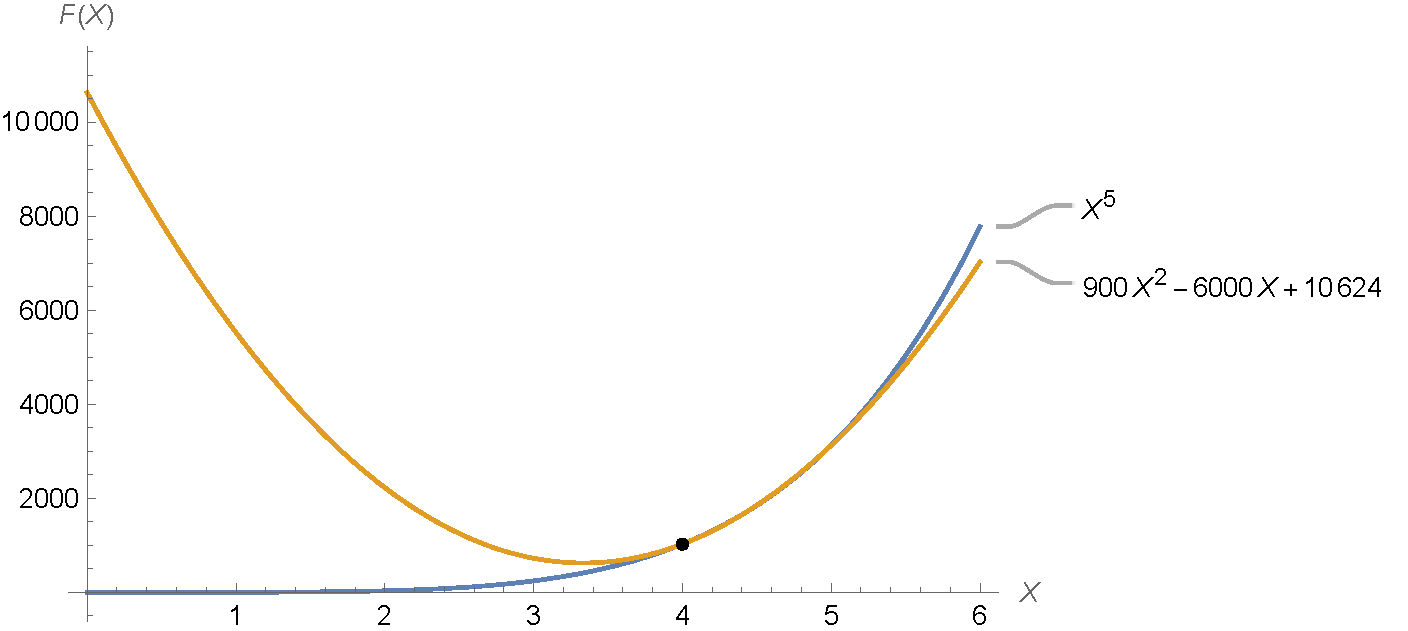
\includegraphics[width=1\textwidth]{sections/images/03_plots_polynomial_p2_n4_with_fifth}
    ~\caption{Approximation of fifth power $X^5$ by $P(2, X, 4)$.
    Points of intersection $X=4$, $X=4.42472$, $X=4.99181$.
    Convergence interval is $4.0 \leq X \leq 5.1$ with percentage error $E < 1\%$.
    }\label{fig:03_plots_polynomial_p2_n4_with_fifth}
\end{figure}
As observed, the polynomial $P(2, X, 4)$ approximates $X^5$ in a certain neighborhood of $N=4$ with
the convergence interval $4.0 \leq X \leq 5.1$ such that the percentage error is less than $1\%$ which is quite remarkable.
The following table presents specific values of absolute, relative, and percentage errors for this approximation
\begin{table}[H]
    \centering
    \begin{tabular}{|c|c|c|c|c|c|}
        \hline
        \textbf{X} & \textbf{$X^5$} & \textbf{$900X^2 - 6000X + 10624$} & \textbf{ABS} & \textbf{Relative} & \textbf{\% Error} \\ \hline
        4.0        & 1024.0         & 1024.0                            & 0.0          & 0.0               & 0.0               \\ \hline
        4.1        & 1158.56        & 1153.0                            & 5.56201      & 0.00480079        & 0.480079          \\ \hline
        4.2        & 1306.91        & 1300.0                            & 6.91232      & 0.00528905        & 0.528905          \\ \hline
        4.3        & 1470.08        & 1465.0                            & 5.08443      & 0.0034586         & 0.34586           \\ \hline
        4.4        & 1649.16        & 1648.0                            & 1.16224      & 0.000704746       & 0.0704746         \\ \hline
        4.5        & 1845.28        & 1849.0                            & 3.71875      & 0.00201528        & 0.201528          \\ \hline
        4.6        & 2059.63        & 2068.0                            & 8.37024      & 0.00406395        & 0.406395          \\ \hline
        4.7        & 2293.45        & 2305.0                            & 11.5499      & 0.00503605        & 0.503605          \\ \hline
        4.8        & 2548.04        & 2560.0                            & 11.9603      & 0.00469393        & 0.469393          \\ \hline
        4.9        & 2824.75        & 2833.0                            & 8.24751      & 0.00291973        & 0.291973          \\ \hline
        5.0        & 3125.0         & 3124.0                            & 1.0          & 0.00032           & 0.032             \\ \hline
        5.1        & 3450.25        & 3433.0                            & 17.2525      & 0.00500036        & 0.500036          \\ \hline
    \end{tabular}
    \caption{Comparison of $X^5$ and $P(2,X,4) = 900X^2 - 6000X + 10624$}
    \label{tab:table2}
\end{table}


One more interesting observation arises by increasing the value of $N$ in $P(m, X, N)$ while keeping $m$ fixed.
As $N$ increases, the length of the convergence interval with the odd-power $X^{2m+1}$ also increases.
For instance,
\begin{itemize}
    \item For $P(2, X, 4)$ and $X^5$, the convergence interval with a percentage error less than $1\%$ is $4.0 \leq X \leq 5.1$, with a length $L=1.1$
    \item For $P(2, X, 20)$ and $X^5$, the convergence interval with a percentage error less than $1\%$ is $18.7 \leq X \leq 22.9$, with a length $L=4.2$
    \item For $P(2, X, 120)$ and $X^5$, the convergence interval with a percentage error less than $1\%$ is $110.0 \leq X \leq 134.7$, with a length $L=24.7$
\end{itemize}

The reason behind this behavior lies in the implicit form of the polynomial $P(m,X,N)$,
meaning that
\begin{align*}
    P(m,X,N) = \sum_{r=0}^{m} (-1)^{m-r} U(m, N, r) \cdot X^{r}
\end{align*}
where $U(m, N, r)$ is a polynomial defined as follows
\begin{align*}
    U(m, N, r) = (-1)^m \sum_{k=1}^{N} \sum_{j=r}^{m} \binom{j}{r} \coeffA{m}{j} k^{2j-r} (-1)^j
\end{align*}
which grows as $N$ increases.
Few cases of coefficients $U(m, N, r)$ are registered as OEIS sequences~\cite{
    oeis_coefficients_u_m_l_k_defined_by_polynomial_identity_1,
    oeis_coefficients_u_m_l_k_defined_by_polynomial_identity_2,
    oeis_coefficients_u_m_l_k_defined_by_polynomial_identity_3}.

To summarize, let us recap the key findings so far.
The polynomial $P(m,X,N)$ is an $m$-degree polynomial in $X \in \mathbb{R}$ with fixed non-negative integers $m$ and $N$.
It approximates the odd power function $X^{2m+1}$ within a specific neighborhood of $N$.
The length $L$ of the convergence interval between $X^{2m+1}$ and $P(m,X,N)$ increases as $N$ grows.

For the sake of clear and precise verification of results, consider the Mathematica programs to generate
plots and data tables, so that reader is able to verify the main results of current part of manuscript,
see~\cite{kolosovpetro_gist}.

So far we have discussed approximation of odd power function $X^{2m+1}$, now we focus on its even case $X^{2m+2}$
which is quite straightforward.
Considering the same example $P(2, X, 4)$ we reach the approximation of even power $X^6$
by means of $K$-times multiplication by $X$, with graphic representation as follows
\begin{figure}[H]
    \centering
    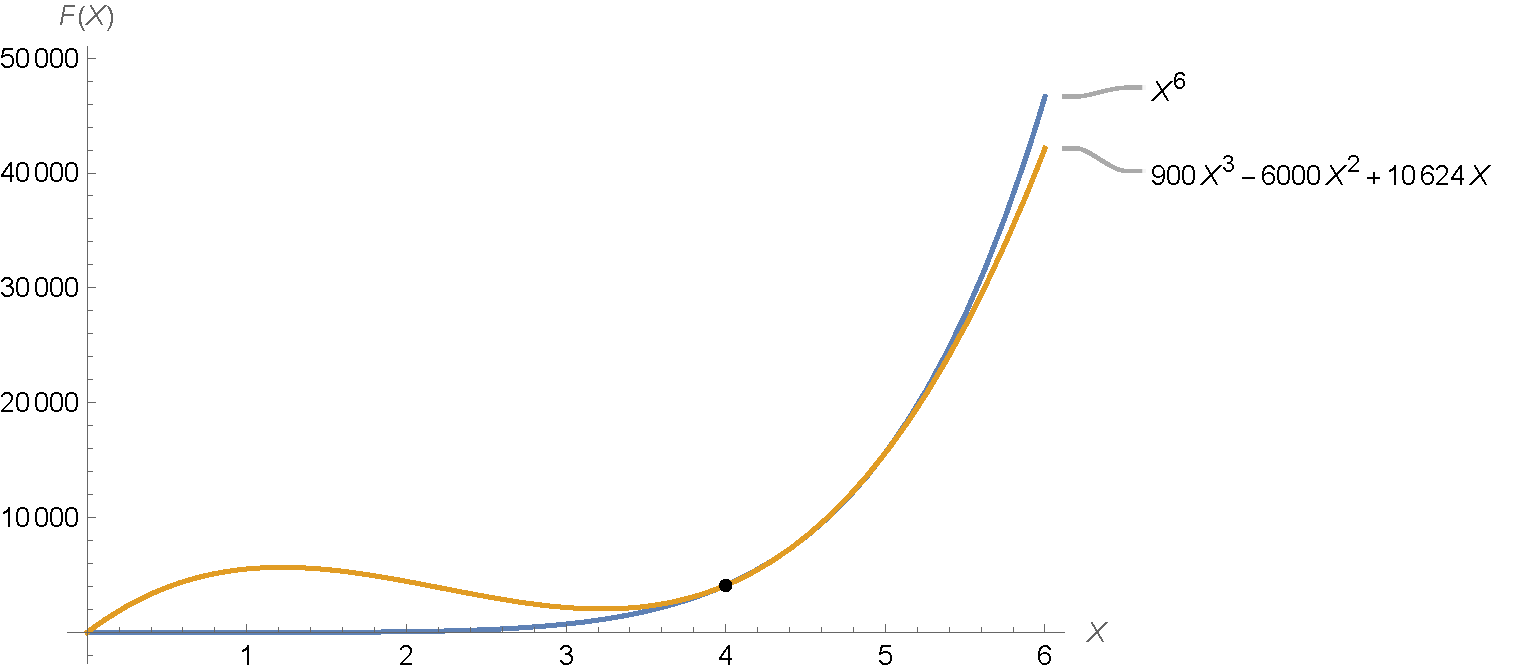
\includegraphics[width=1\textwidth]{sections/images/07_plot_of_6th_power_with_p_2_4_times_x}
    ~\caption{Approximation of sixth power $X^6$ by $P(2, X, 4) \cdot X$.
    Convergence interval is $3.9 \leq X \leq 5.1$ with percentage error $E < 3\%$.
    }\label{fig:07_plot_of_6th_power_with_p_2_4_times_x}
\end{figure}
Therefore, we have reached the statement that
the polynomial $P(m,X,N)$ is an $m$-degree polynomial in $X$, having fixed non-negative
integers $m$ and $N$.
It approximates the power function $X^{j}$ in a certain neighborhood of fixed $N$.
The length of convergence interval between the power function $X^j$ and $P(m,X,N) \cdot X^K$ increases as $N$ grow.
